\chapter{Data processing with Spark}
%Intro\footnotemark\\
\par Spark can be used to perform complex processing on HBase data. In this Chapter, the different "Executors" of Spark will be co-located with the regions
servers, and will be able to carry out parallel processing directly where the data is stored.
\begin{spacing}{1.2}
%note en bas de page
\section{Preparation of the environment }
\par First of all we download and install Apache Maven
\\
\begin{figure}[!htb] 
\begin{center} 
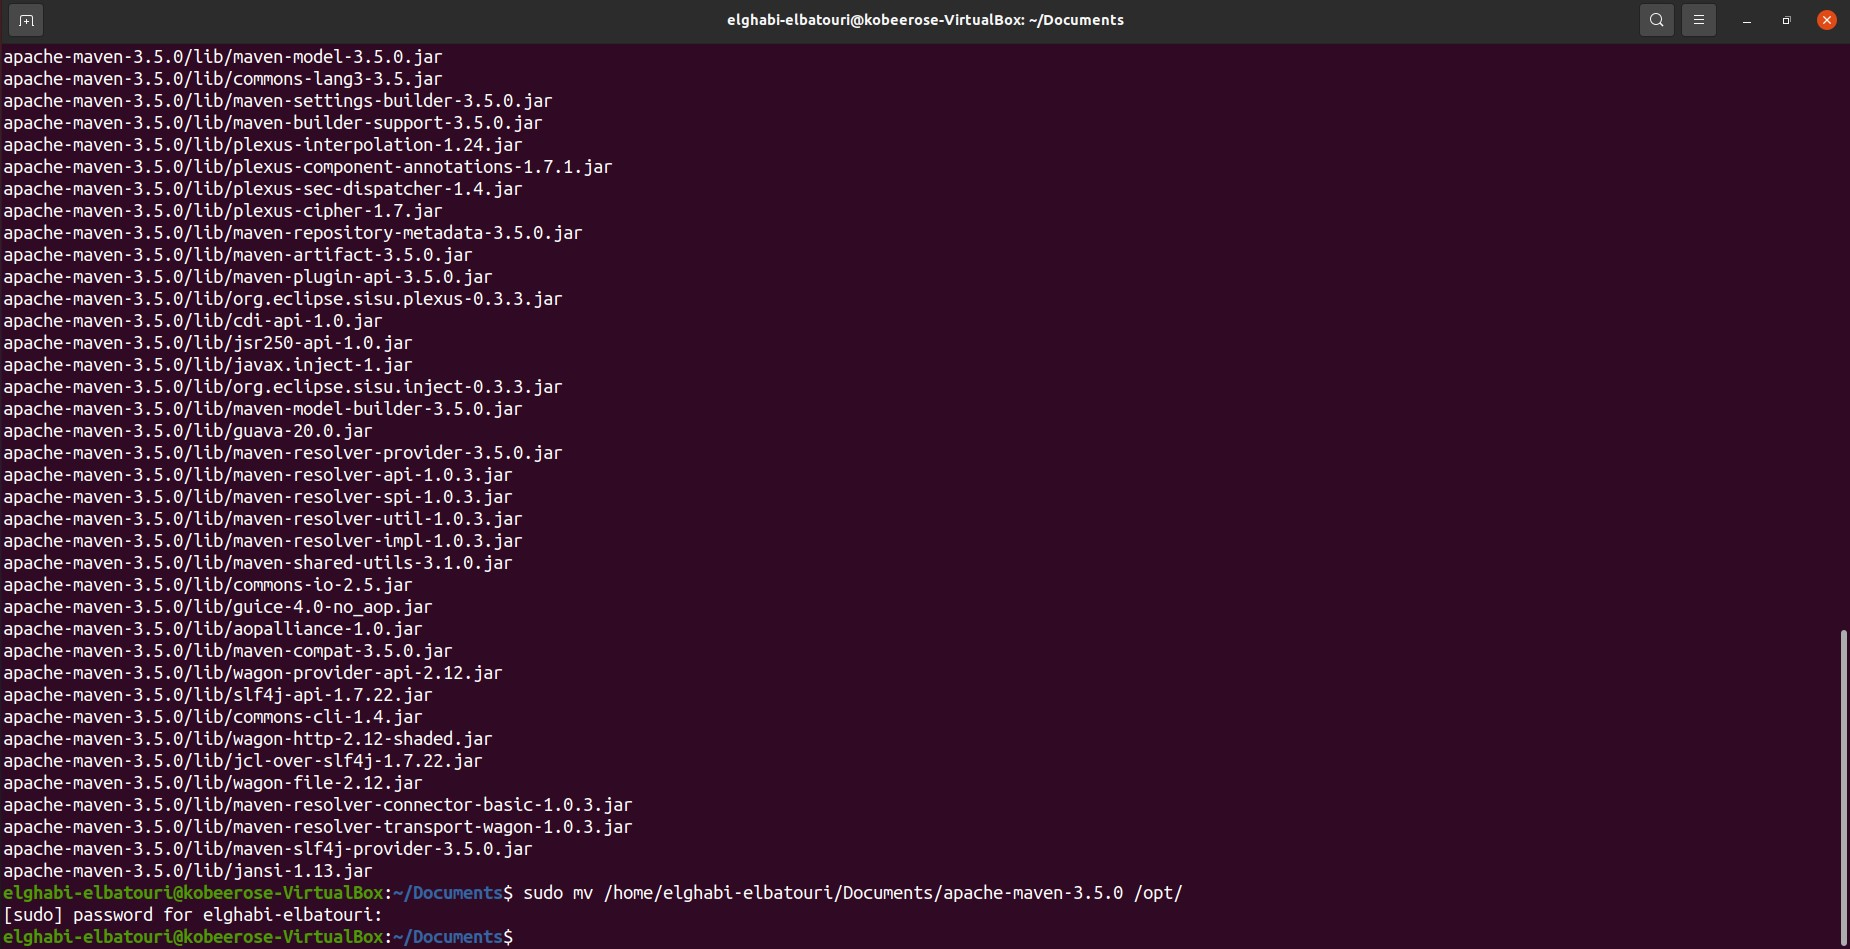
\includegraphics[width=1\linewidth]{Pictures/HBase/Data processing with Spark/Preparation of the environment/Installing Apache Maven} 
\end{center} 
\caption{Installing Apache Maven} 
\end{figure}  \FloatBarrier
\\
\newpage
\par To permanently set up the PATH environment variable for all users. We modify: /etc/profile file by adding the path where the bin of maven in export PATH.
\\
\begin{figure}[!htb] 
\begin{center} 
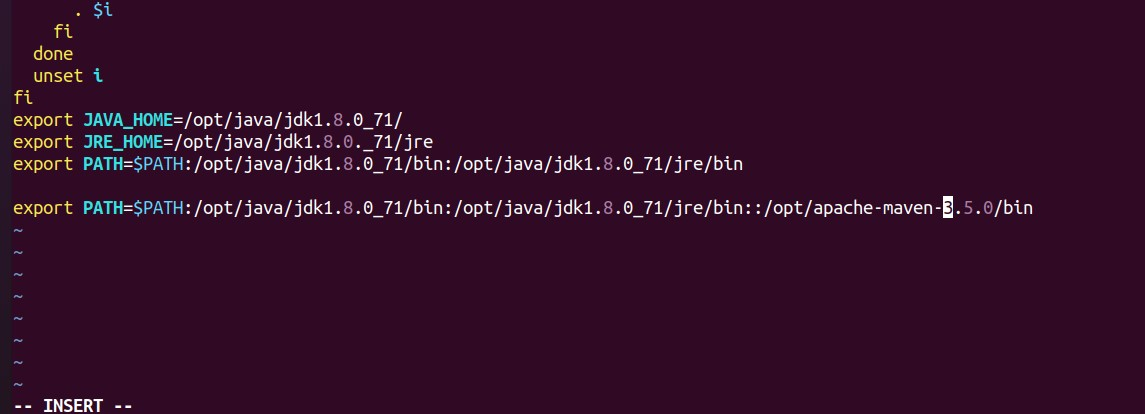
\includegraphics[width=1\linewidth]{Pictures/HBase/Data processing with Spark/Preparation of the environment/Adding Maven to PATH} 
\end{center} 
\caption{Adding Maven to PATH} 
\end{figure}  \FloatBarrier
\\

\par After saving the profile file, we run the source command, then we verify by running mvn -v command.
\\
\begin{figure}[!htb] 
\begin{center} 
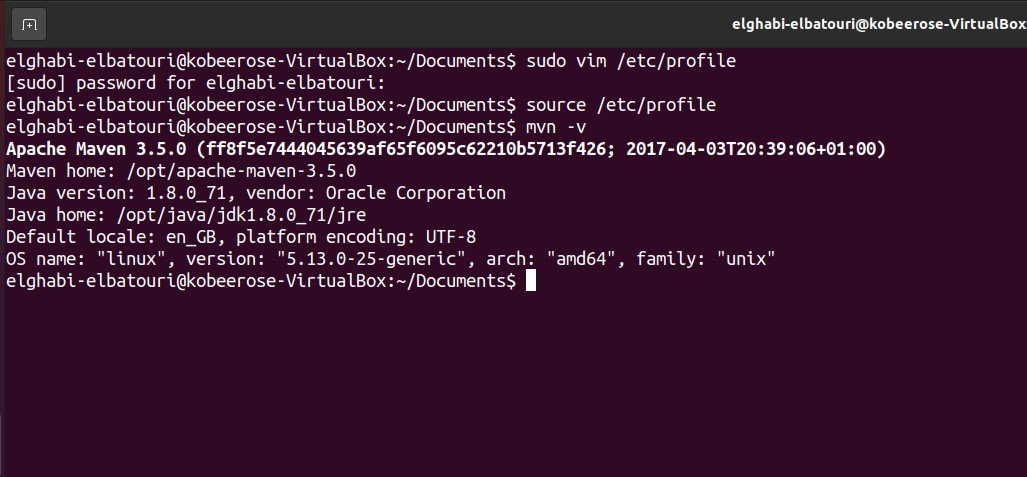
\includegraphics[width=1\linewidth]{Pictures/HBase/Data processing with Spark/Preparation of the environment/Checking mvn -v command} 
\end{center} 
\caption{Checking mvn -v command} 
\end{figure}  \FloatBarrier
\\
\newpage
\par Let's create a Maven project. As we can see at the end of the maven project generation, a "Build success" message is displayed.
\\
\begin{figure}[!htb] 
\begin{center} 
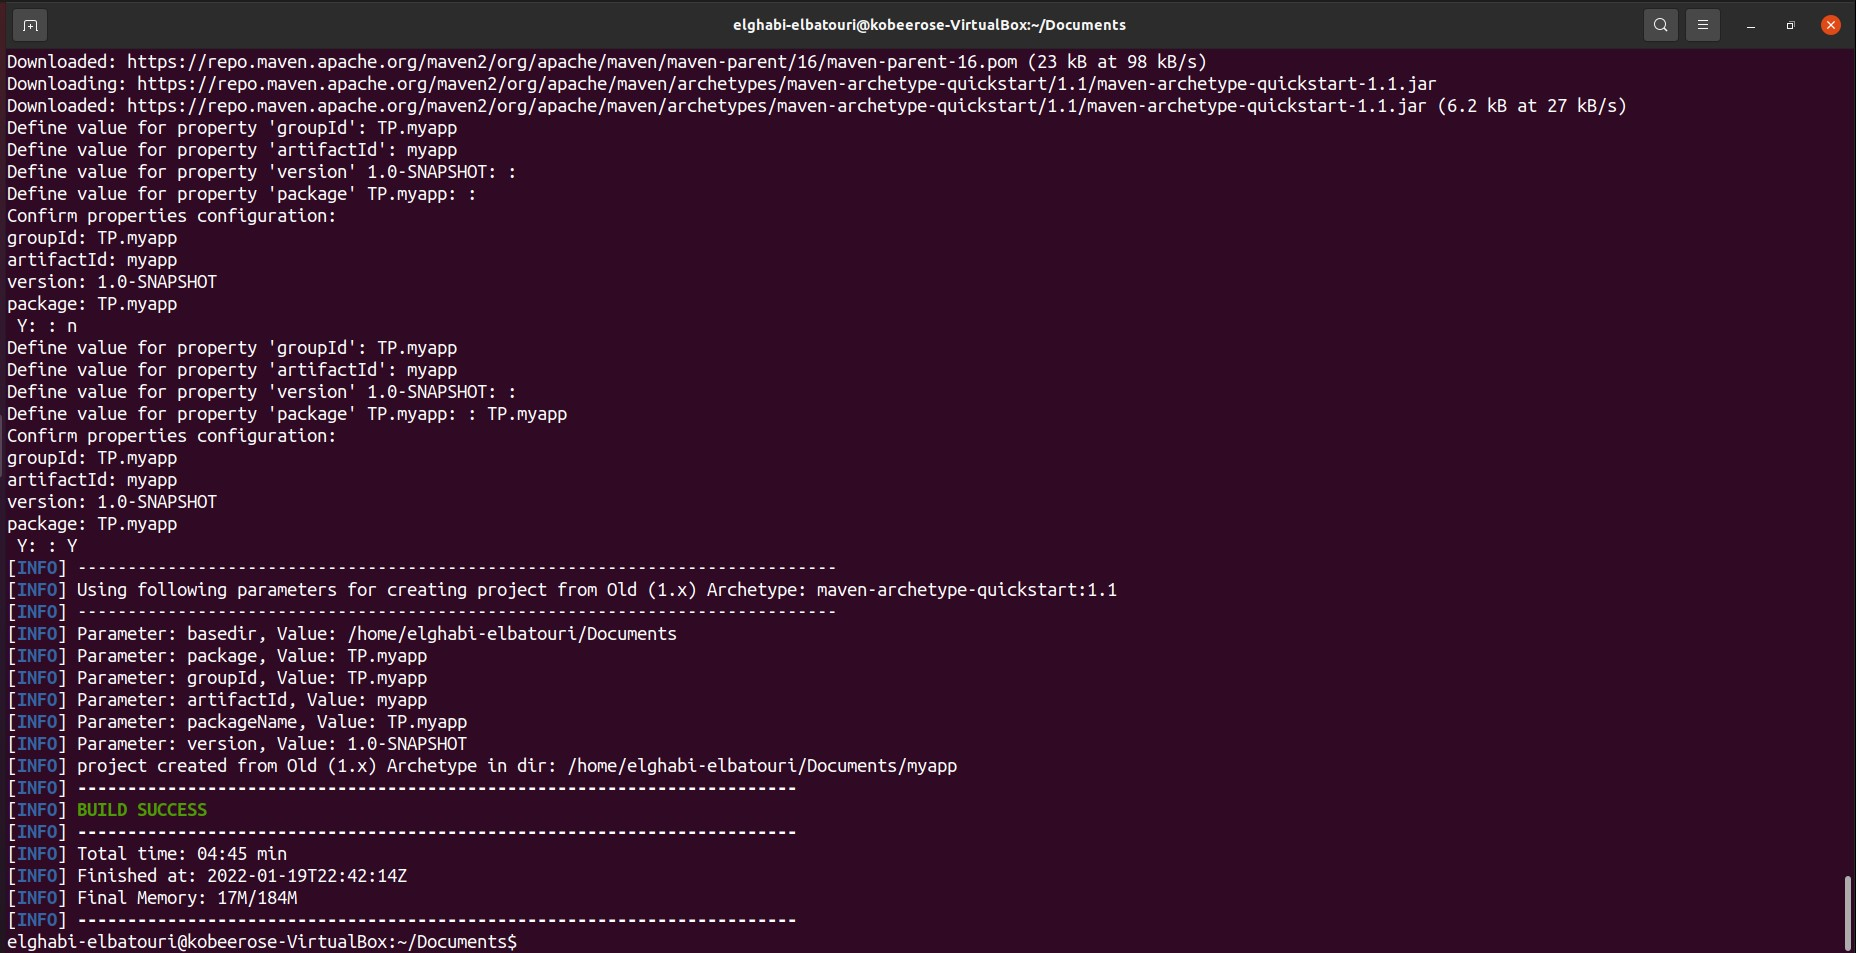
\includegraphics[width=1\linewidth]{Pictures/HBase/Data processing with Spark/Preparation of the environment/Creating Maven project} 
\end{center} 
\caption{Creating Maven project} 
\end{figure}  \FloatBarrier
\\

\par Reconfiguring the Maven project by modifying the pom.xml file to add dependencies and build properties.
\\
\begin{figure}[!htb] 
\begin{center} 
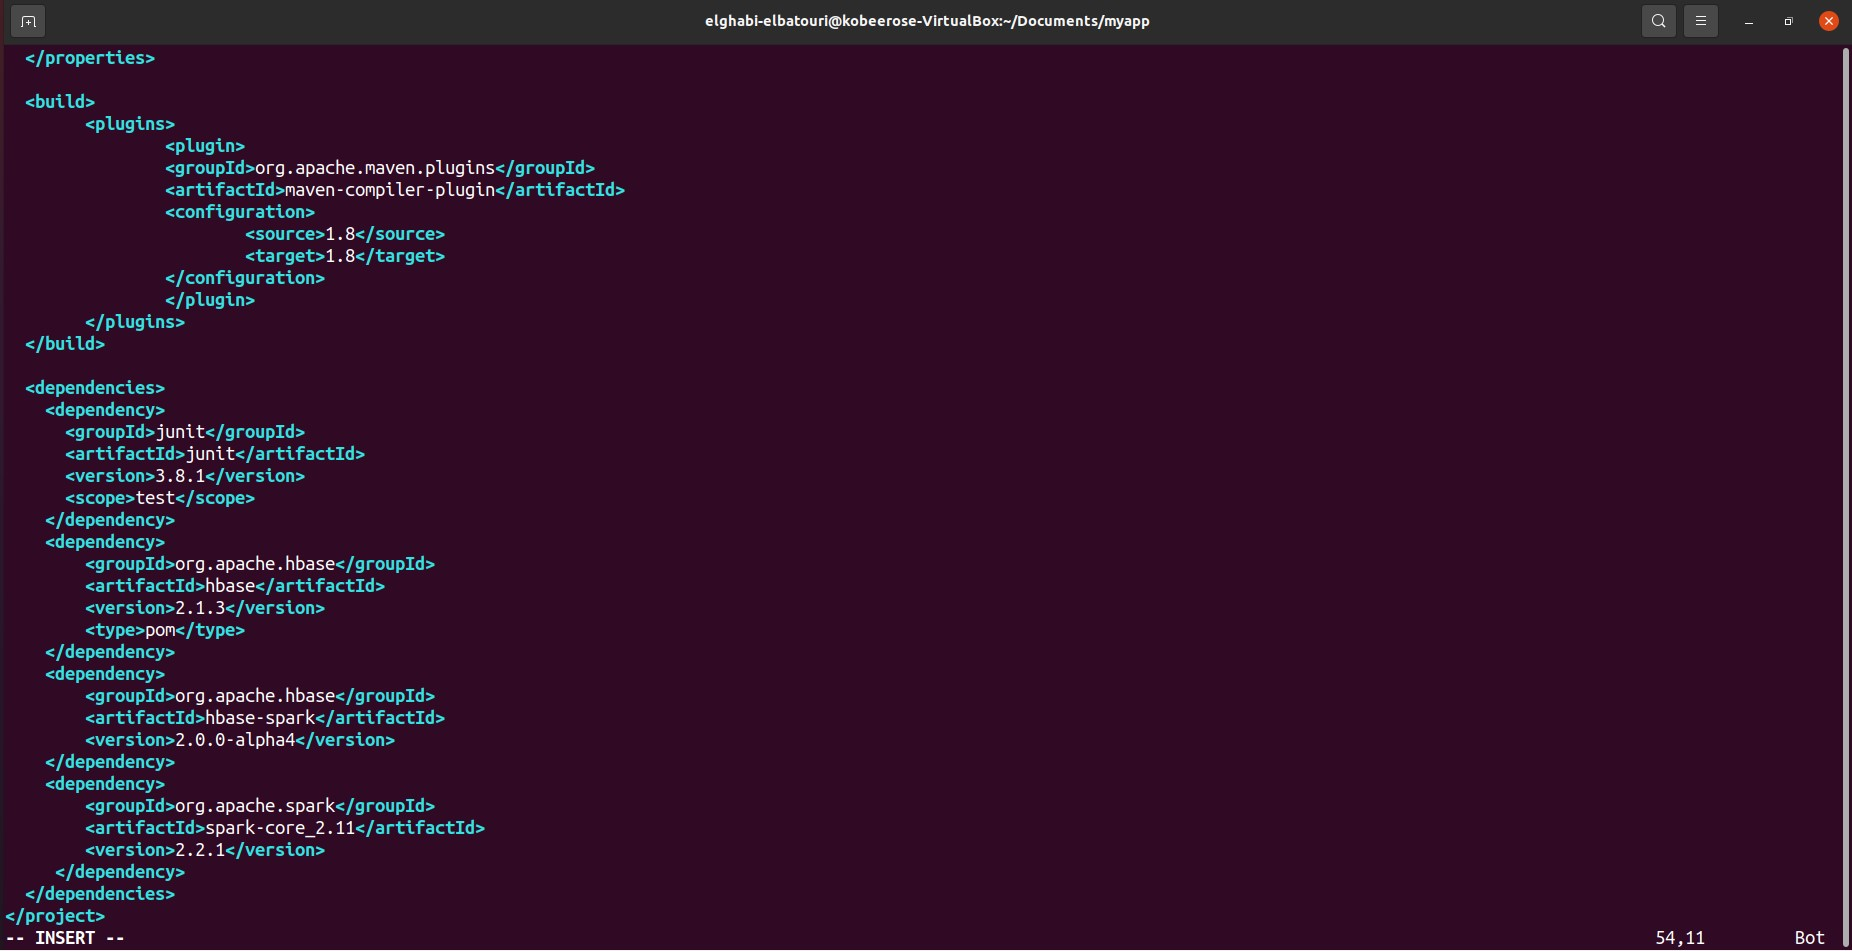
\includegraphics[width=1\linewidth]{Pictures/HBase/Data processing with Spark/Preparation of the environment/Configuring pom.xml} 
\end{center} 
\caption{Configuring pom.xml} 
\end{figure}  \FloatBarrier
\\
\newpage
\par Implementing the "WordCountTask" process in the “HbaseSparkProcess.java” file.
\\
\begin{figure}[!htb] 
\begin{center} 
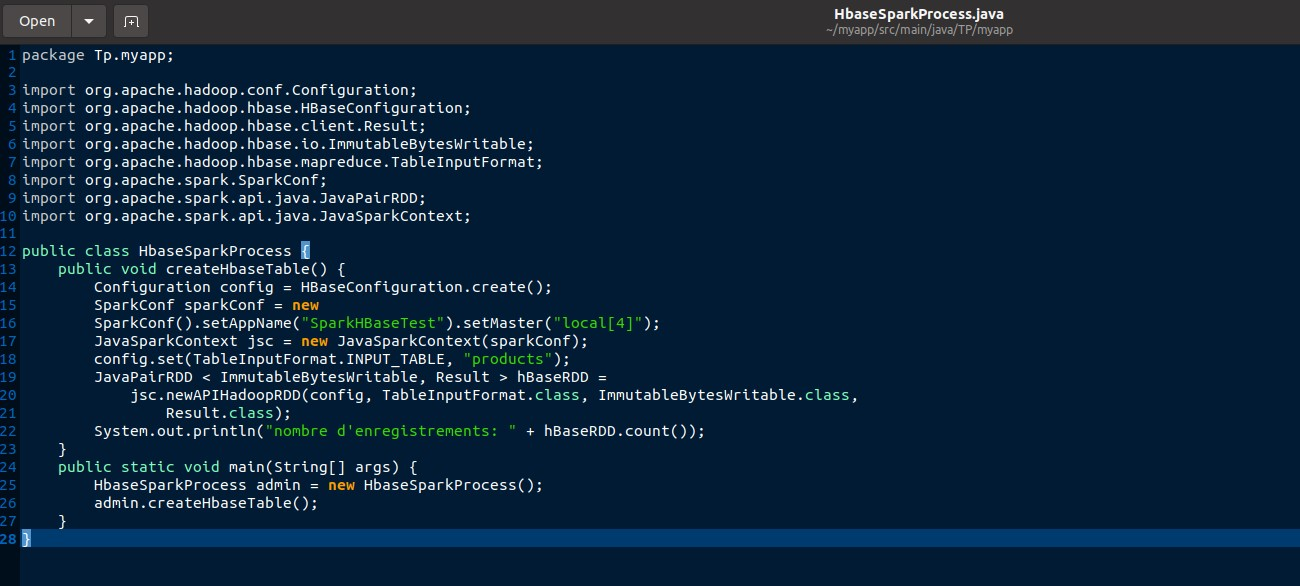
\includegraphics[width=1\linewidth]{Pictures/HBase/Data processing with Spark/Preparation of the environment/Creating HbaseSparkProcess.java file} 
\end{center} 
\caption{Creating HbaseSparkProcess.java file} 
\end{figure}  \FloatBarrier
\\

\par Making an mvn install package on the project. A myapp-1.0-SNAPSHOT.jar file will be created in the target directory of the project.
\\
\begin{figure}[!htb] 
\begin{center} 
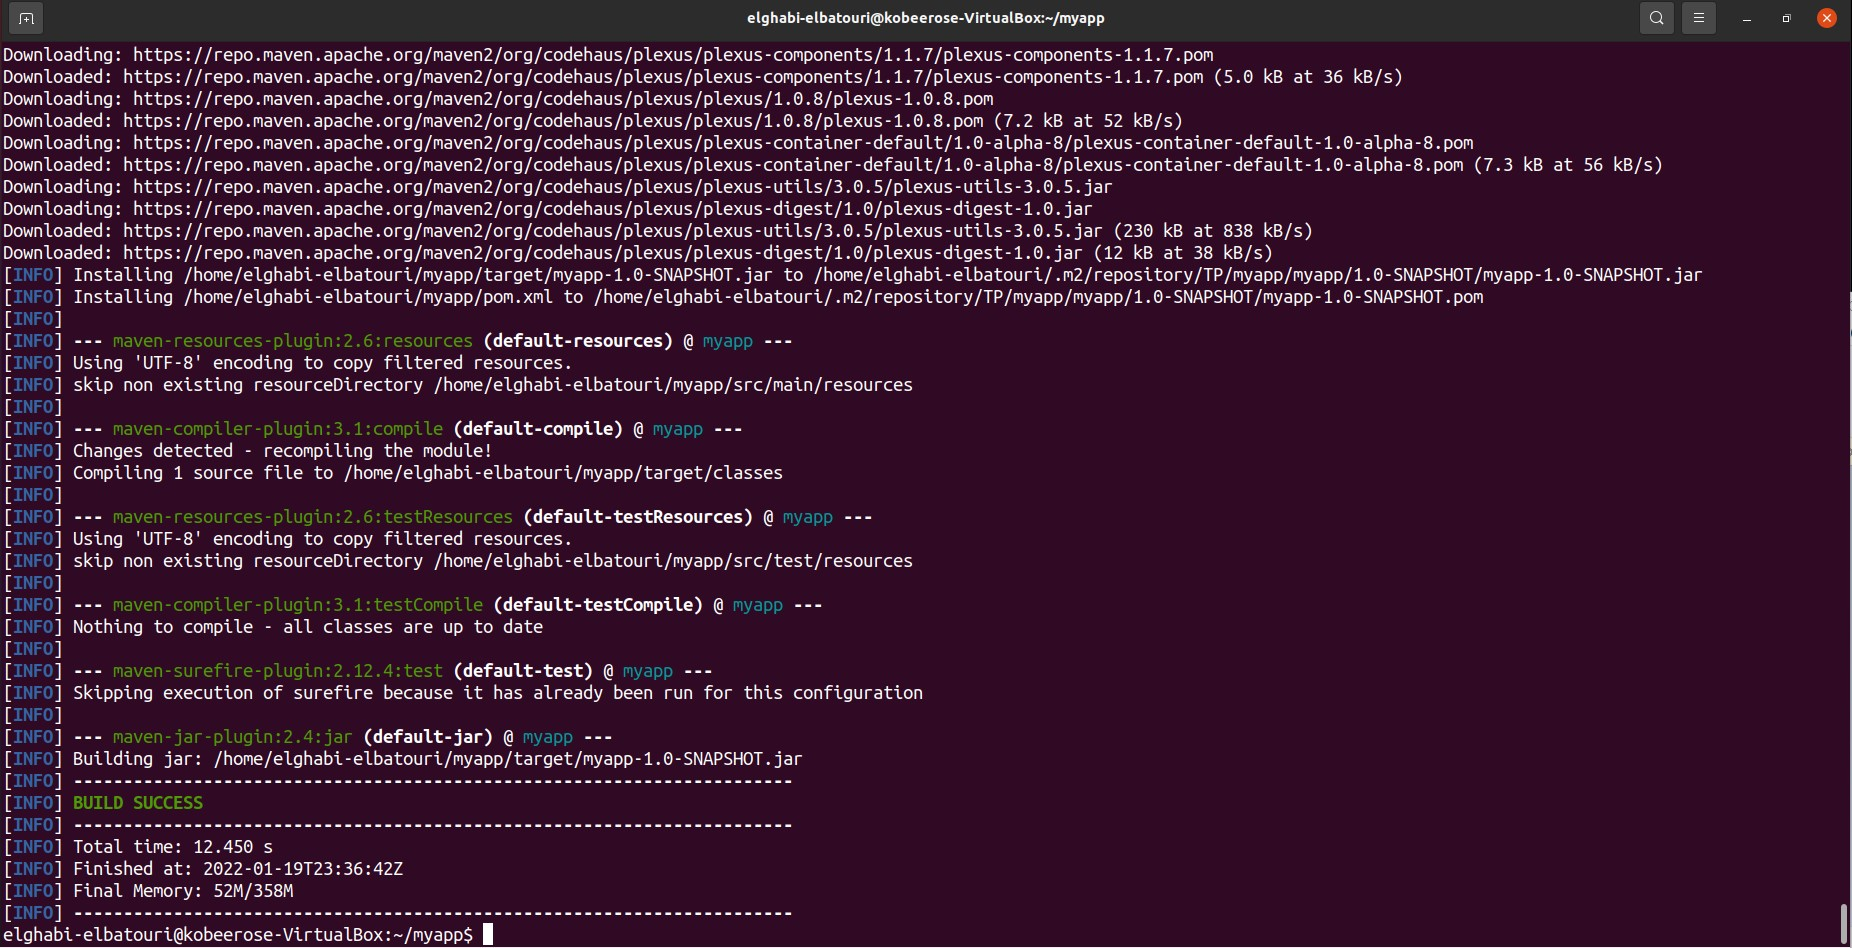
\includegraphics[width=1\linewidth]{Pictures/HBase/Data processing with Spark/Preparation of the environment/mvn install package command} 
\end{center} 
\caption{mvn install package command} 
\end{figure}  \FloatBarrier
\\
\newpage
\section{Installing and Configuring Spark-2.4.3 }
\par We start by Downloading version spark-2.4.3-bin-hadoop2.7.tgz, Unziping the recovered file then werename it and place it in the /usr/local directory.
\\
\begin{figure}[!htb] 
\begin{center} 
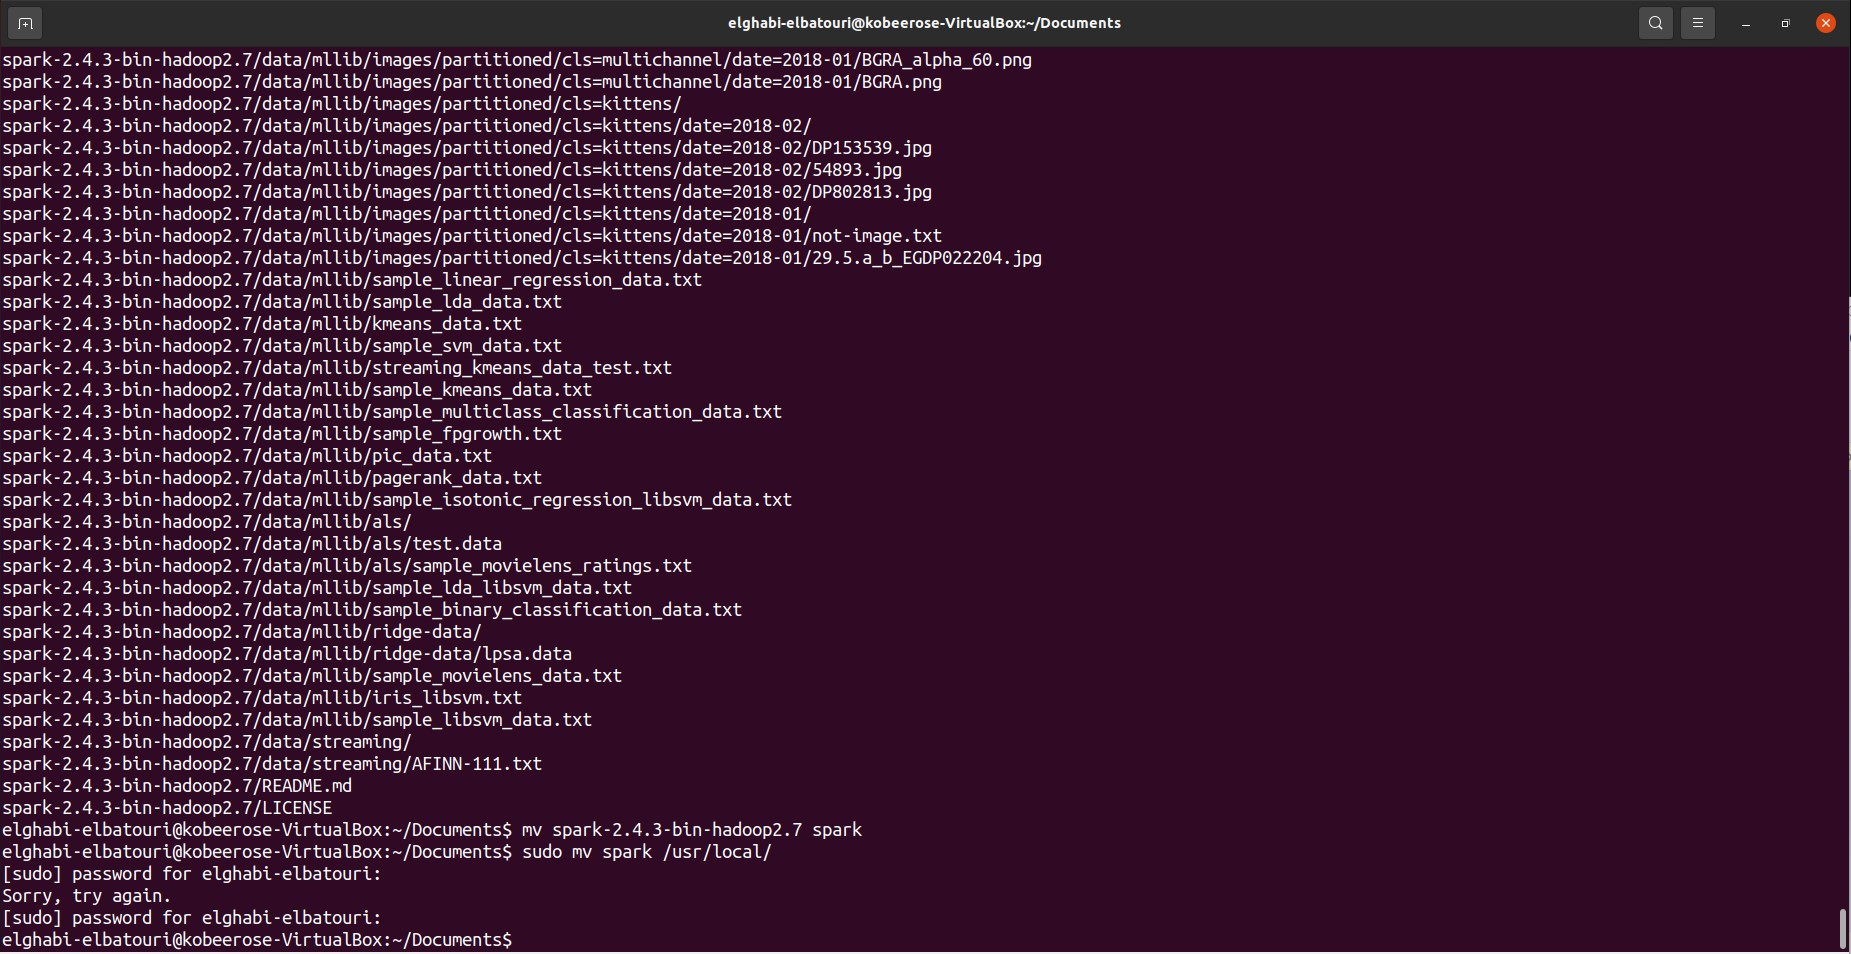
\includegraphics[width=1\linewidth]{Pictures/HBase/Data processing with Spark/Installing and Configuring Spark-2.4.3/Download and Extract Spark} 
\end{center} 
\caption{Download and Extract Spark} 
\end{figure}  \FloatBarrier
\\

\par Open the .bashrc file and modify the PATH by adding the path where the bin is located
by spark.
\\
\begin{figure}[!htb] 
\begin{center} 
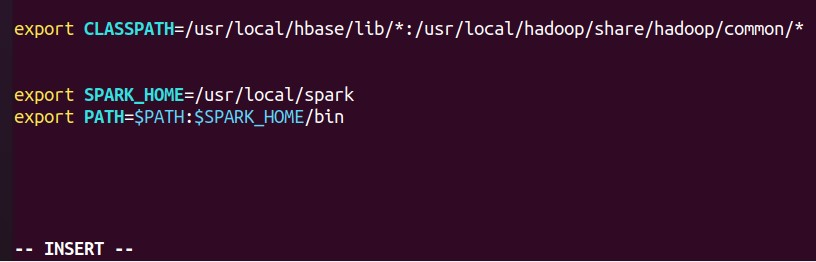
\includegraphics[width=1\linewidth]{Pictures/HBase/Data processing with Spark/Installing and Configuring Spark-2.4.3/Adding Spark to PATH Variable} 
\end{center} 
\caption{Adding Spark to PATH Variable} 
\end{figure}  \FloatBarrier
\\
\newpage
\par We should also install Python before going forward with the project.
\\
\begin{figure}[!htb] 
\begin{center} 
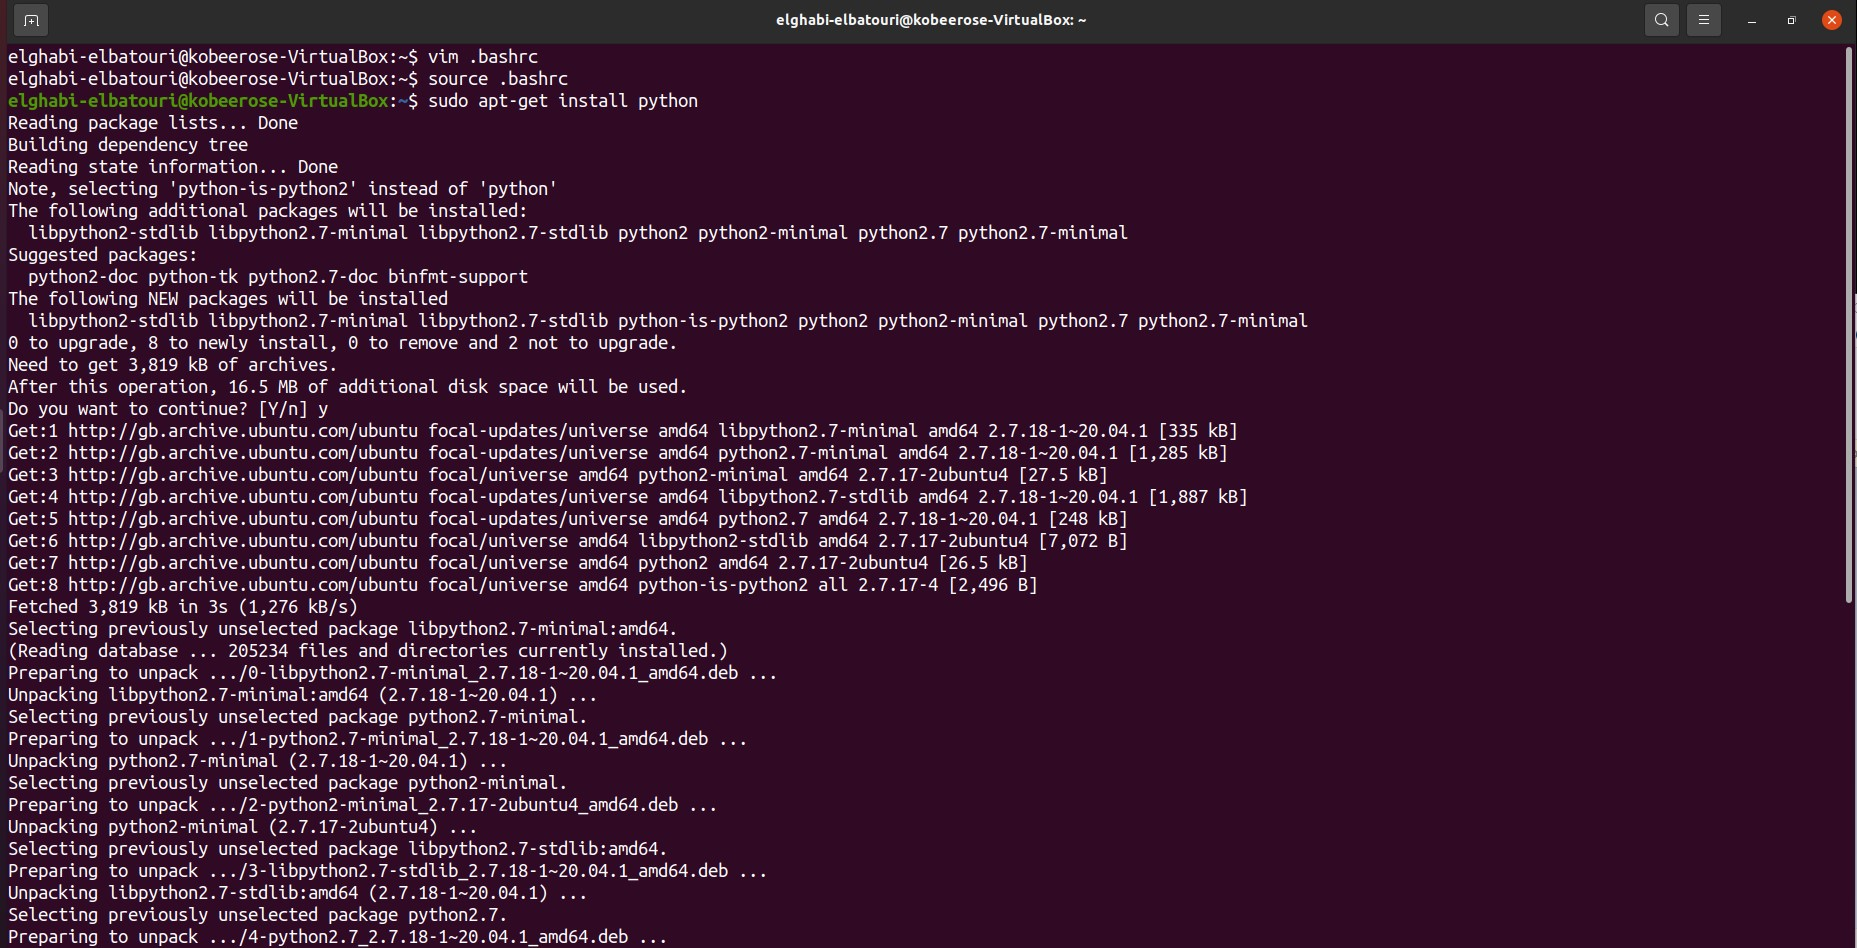
\includegraphics[width=1\linewidth]{Pictures/HBase/Data processing with Spark/Installing and Configuring Spark-2.4.3/Installing Python} 
\end{center} 
\caption{Installing Python} 
\end{figure}  \FloatBarrier
\\

\par We configure spark-env.sh file to ensure connection Spark to a Hadoop distribution.
\\
\begin{figure}[!htb] 
\begin{center} 
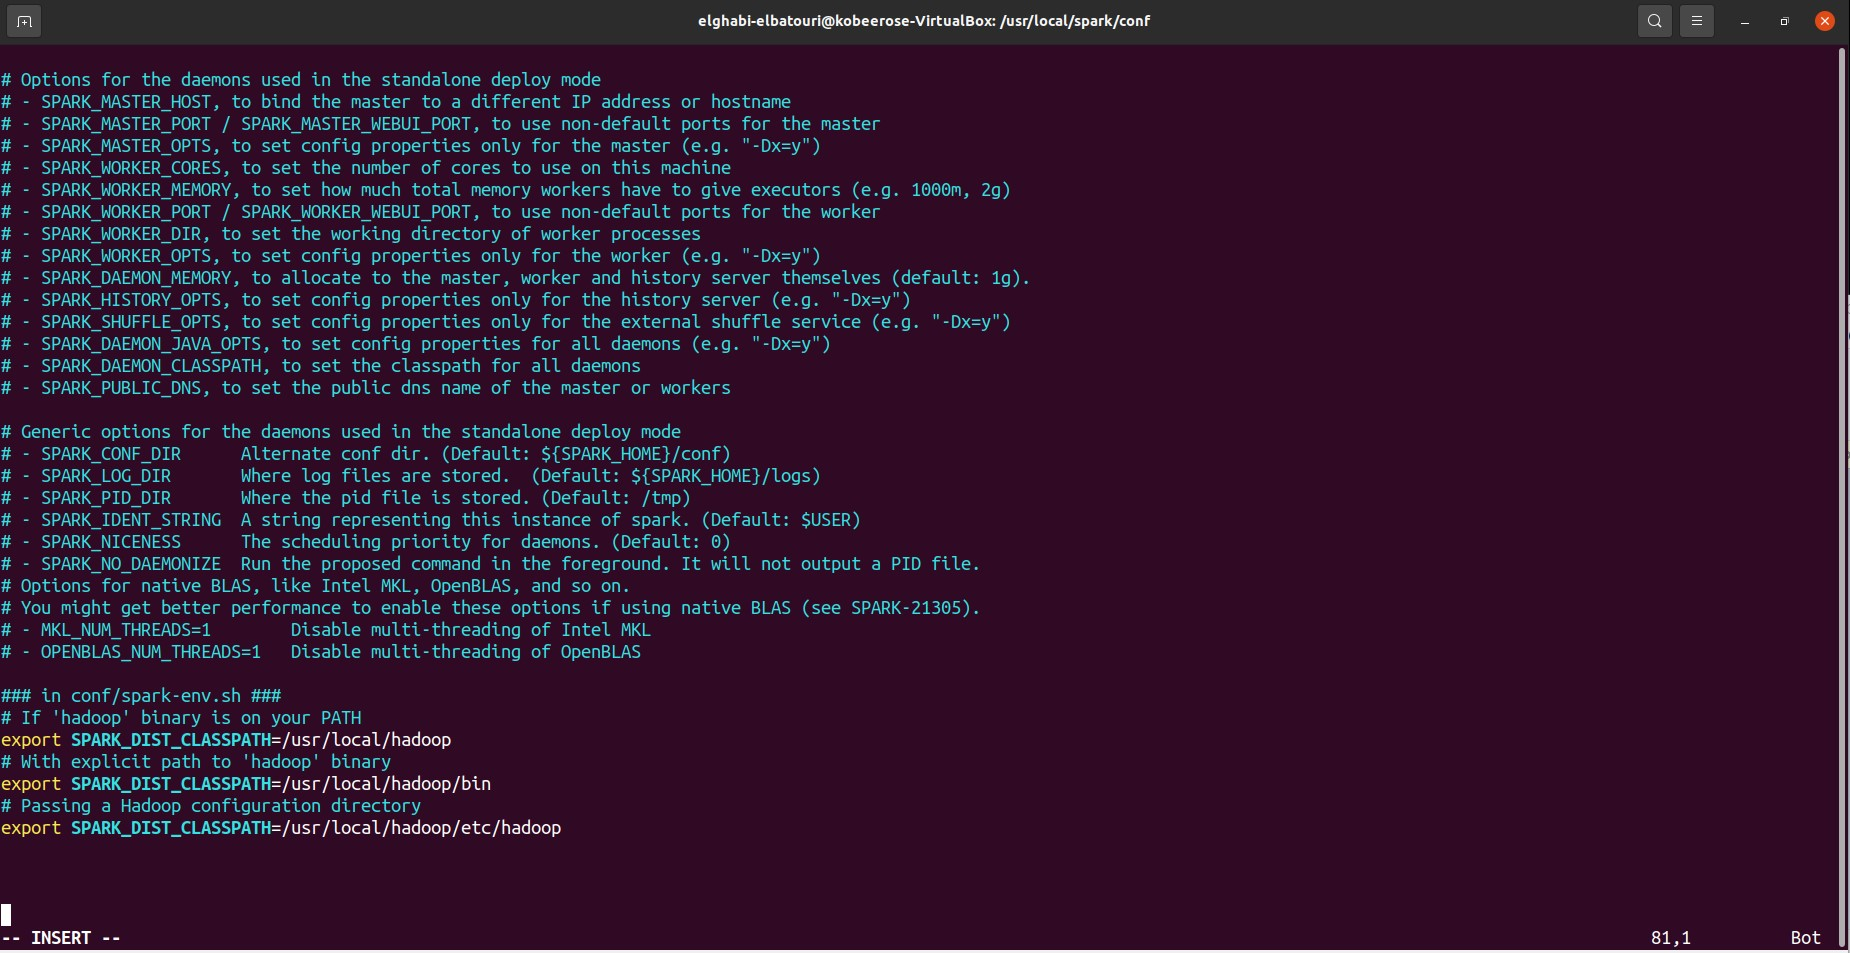
\includegraphics[width=1\linewidth]{Pictures/HBase/Data processing with Spark/Installing and Configuring Spark-2.4.3/Configuring spark-env.sh file} 
\end{center} 
\caption{Configuring spark-env.sh file} 
\end{figure}  \FloatBarrier
\\
\newpage
\par Then we copy the myapp-1.0-SNAPSHOT.jar file to our /usr/local/spark directory.
\\
\begin{figure}[!htb] 
\begin{center} 
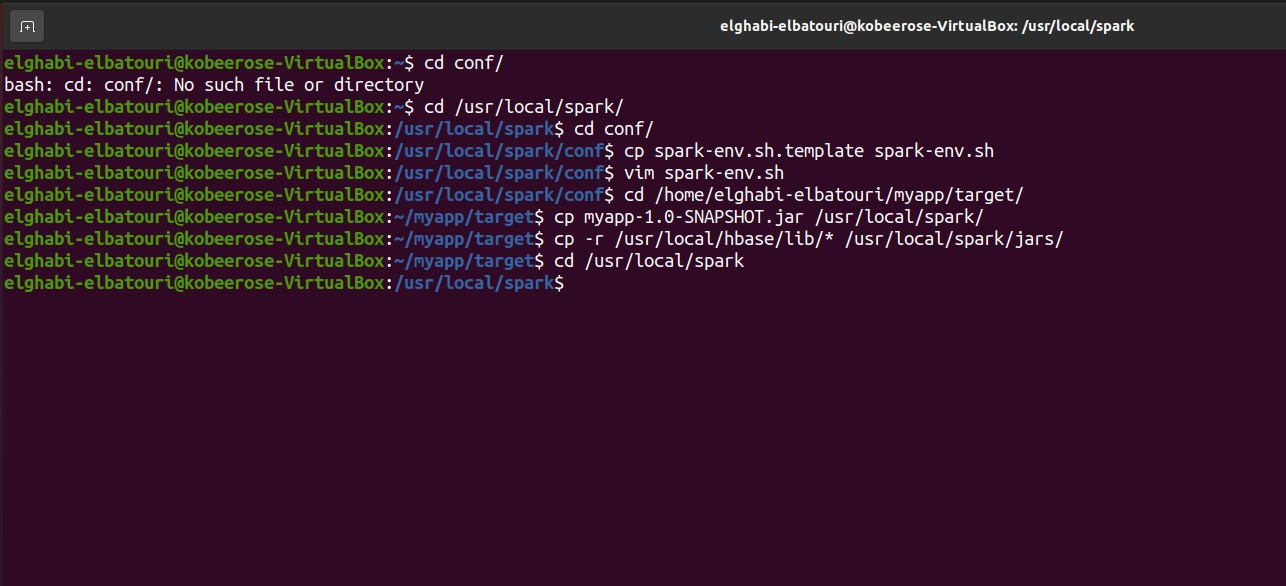
\includegraphics[width=1\linewidth]{Pictures/HBase/Data processing with Spark/Installing and Configuring Spark-2.4.3/Copying myapp to Spark directory} 
\end{center} 
\caption{Copying myapp to Spark directory} 
\end{figure}  \FloatBarrier
\\

\par Finally we run this file through spark-submit.
\\
\begin{figure}[!htb] 
\begin{center} 
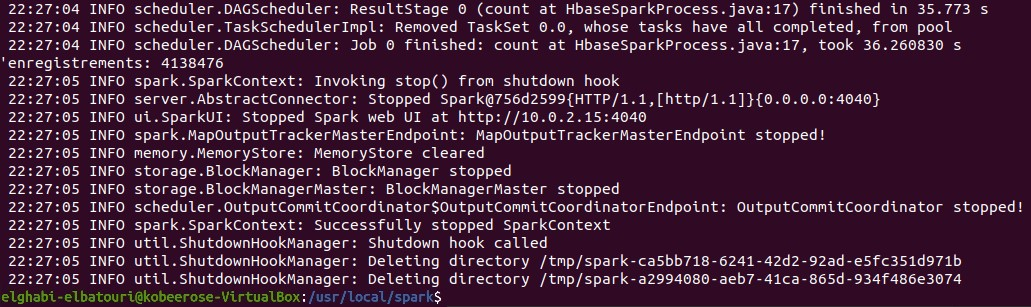
\includegraphics[width=1\linewidth]{Pictures/HBase/Data processing with Spark/Installing and Configuring Spark-2.4.3/Spark submit command} 
\end{center} 
\caption{Spark submit command} 
\end{figure}  \FloatBarrier
\\

\end{spacing}